\documentclass[tikz,border=10pt]{standalone}

\begin{document}
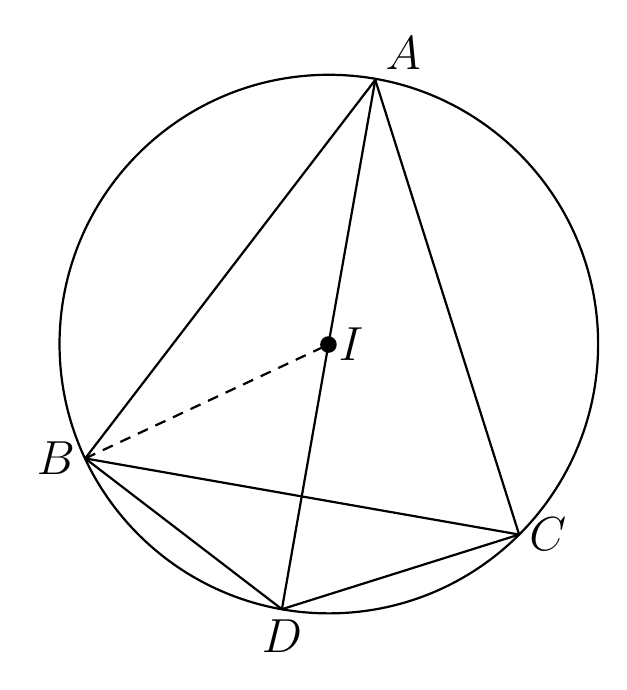
\begin{tikzpicture}[line width=0.8pt, line join=round,
  every node/.style={font=\fontsize{17.5}{21}\selectfont}]
\coordinate (A) at (0.865,3.370);
\coordinate (B) at (-2.819,-1.437);
\coordinate (C) at (2.692,-2.404);
\coordinate (D) at (-0.321,-3.352);
\coordinate (I) at (0.270,0.009);








  
  \draw (0.275,0.015) circle (3.420);

  
  \draw (A) -- (B) -- (C) -- (D);
  \draw (A) -- (I) -- (D);

  
  \draw (A) -- (C);
  \draw (B) -- (D);

  
  \draw[dash pattern=on 4pt off 3pt] (B) -- (I);

  
  \fill (I) circle (3.000pt);

  \node[above right] at (A) {$A$};
  \node[left] at (B) {$B$};
  \node[right] at (C) {$C$};
  \node[below] at (D) {$D$};
  \node[right] at (I) {$I$};
\end{tikzpicture}
\end{document}